\documentclass[conference]{IEEEtran}
\IEEEoverridecommandlockouts
% The preceding line is only needed to identify funding in the first footnote. If that is unneeded, please comment it out.
\usepackage{cite}
\usepackage{amsmath,amssymb,amsfonts}
\usepackage{algorithmic}
\usepackage{graphicx}
\usepackage{textcomp}
\usepackage{xcolor}
\usepackage{hyperref}
\usepackage{float}
\usepackage[ngerman]{babel}
\def\BibTeX{{\rm B\kern-.05em{\sc i\kern-.025em b}\kern-.08em
    T\kern-.1667em\lower.7ex\hbox{E}\kern-.125emX}}
\begin{document}

\title{Dokumentation der Softwarearchitektur des Projekts Twitter-Dash}

% Authoren	
\author{
    \IEEEauthorblockN{Hahn, Bastian}
    \IEEEauthorblockA{
        \textit{b.hahn@oth-aw.de}\\
    }
    \and

    \IEEEauthorblockN{Kleber, Martin}
    \IEEEauthorblockA{
        \textit{m.kleber2@oth-aw.de}\\
    }
    \and

    \IEEEauthorblockN{Klier, Andreas}
    \IEEEauthorblockA{
        \textit{a.klier@oth-aw.de}\\
    }
    \and

    \IEEEauthorblockN{Kreussel, Lukas}
    \IEEEauthorblockA{
        \textit{l.kreussel@oth-aw.de}\\
    }
    \and

    \IEEEauthorblockN{Paris, Felix}
    \IEEEauthorblockA{
        \textit{f.paris1@oth-aw.de}\\
    }
    \and

    \IEEEauthorblockN{Ziegler, Andreas}
    \IEEEauthorblockA{
        \textit{a.ziegler1@oth-aw.de}\\
    }
}

\maketitle

\begin{abstract}
    In diesem technischen Report wird die Softwarearchitektur des Projekts
    Twitter-Dash vorgestellt. Das Projekt wurde im Rahmen der Vorlesung
    Big Data and Cloud Computing (BDCC) implementiert. Ziel der Implementierung ist es,
    ein Dashboard zu erstellen, welches aktuelle und historische Informationen zu Twitter Trends
    anzeigen und analysieren kann.
\end{abstract}

\begin{IEEEkeywords}
    Twitter, Big Data, Database, Web UI, Data Analysis
\end{IEEEkeywords}

\section{Introduction}
Bei der Applikation Twitter-Dash werden von der Twitter-API alle 15 Minuten die aktuellen Trends
abgegriffen und in einer lokalen Datenbank gespeichert. Die Kommunikation zwischen den
einzelnen Services ist über eine gRPC-Schnittstelle realisiert.
Die Interaktion des Anwenders mit der Applikation erfolgt dabei über eine Web-UI basierend auf dem
React Web-Framework.

\section{Architektur Allgemein}

Als Architektur wird ein Ansatz verfolgt, der sich stark an Microservices orientiert.
Dadurch wird eine abgeschlossene Logik von Front- und Backendkomponenten erreicht, die jeweils
von einem Subteam entwickelt wird. Diese gekapselten Einheiten können jeweils als isolierte Applikation der Containervirtualisierung Docker betrieben werden.
Durch eine zentrale Konfigurationsdatei des Containers können diese zwischen den Teammitgliedern
ausgetauscht und ausgeführt werden. Damit wird eine hohe Portabilität gewährleistet.
Die Kommunikation der Teilsysteme wird durch eine sprachunabhängige gRPC-Schnittstelle angeboten.
Dadurch wird es möglich einzelne Komponenten des Gesamtsystems auszutauschen,
ohne größere Veränderungen an den anderen Microservices vornehmen zu müssen \cite{microservices}.

\begin{figure}
    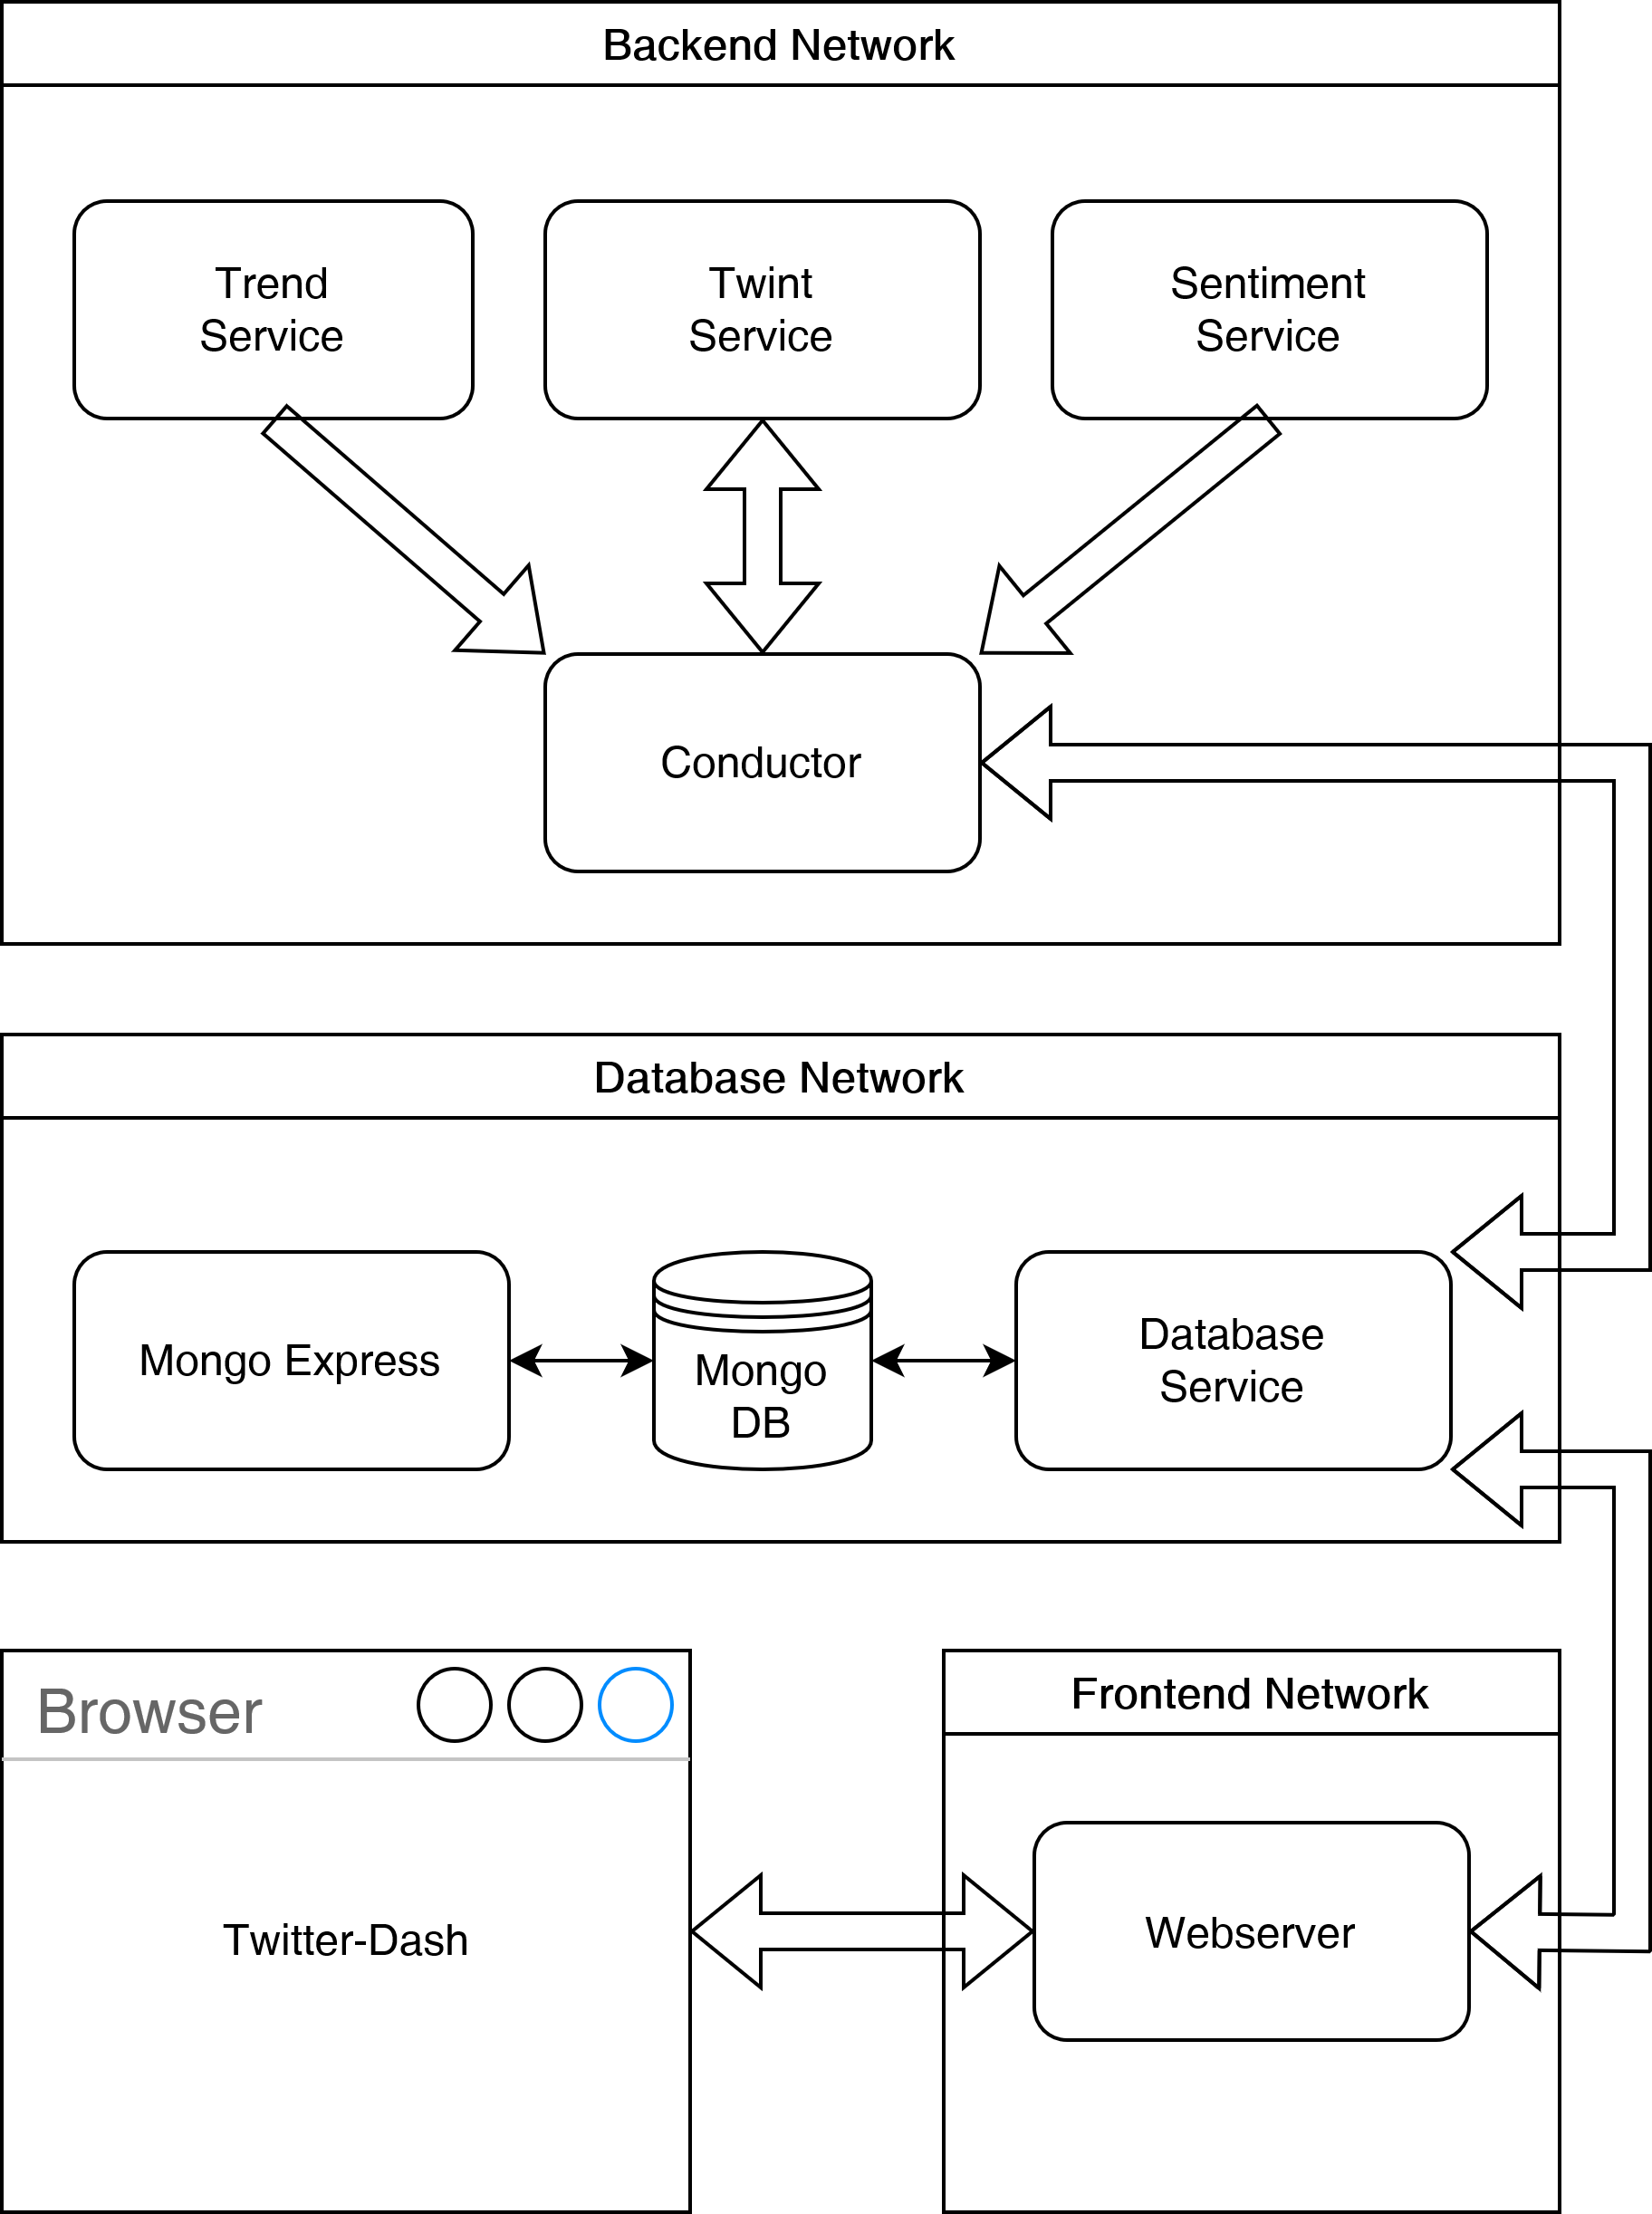
\includegraphics[width=0.5\textwidth]{Architecture.png}
    \caption{Übersicht Gesamtsystem}
\end{figure}


\section{Kommunikation}
Um Konflikten zwischen den Schnittstellendefinitionen der einzelnen Dienste zu vermeiden,
wurden alle gRPC-Schnittstellen in einem globalen Ordner definiert und vor dem Ausführen der Container über ein Script in die jeweiligen Source-Verzeichnisse der Dienste kopiert, bzw. wenn nötig mit dem gRPC-Tool kompiliert.
Dadurch werden Änderungen an den Schnittstellen gleichzeitig für alle Dienste vorgenommen.

%TODO Frontend


\section{Datenakquise}
Um Daten für das Dashboard zu erhalten, werden zwei unterschiedliche Vorgehensweisen verwendet.
Der meist verwendete Ansatz ist die Abfrage über die offizielle Twitter-API \cite{twitterapi}.
Über diese werden die aktuellen Hashtags periodisch abgerufen.
Außerdem wurde Twint, ein fortschrittliches Scraping-Tool verwendet.
Dieses Tool liefert vollständige Tweets, inklusive zugehöriger Meta-Daten,
ohne direkten Zugriff auf die Twitter-API zu benötigen \cite{twint}.

\newpage 

\subsection*{Trend-Service}
Für den Zugriff auf die Twitter-API wurde die Python-Bibliothek Tweepy \cite{tweepy} verwendet.
Diese Bibliothek bietet einen Client für die Verbindung zur Twitter-API.
Über diesen Client werden alle 15 Minuten die aktuellen Trends pro Land abgefragt und nach Hashtags gefiltert.
Diese werden über den Conductor zur Speicherung an die Datenbank gesendet.

Der Trend-Service bietet folgende Funktionen:
\begin{itemize}
    \item OnNewTrends:\newline Löst alle 15 Minuten ein Event aus, welches die aktuellen Hashtags in einer Liste enthält. Die Listenelemente umfassen:
          \begin{itemize}
              \item Hashtag
              \item Platzierung nach Aktualität im Land
              \item Anzahl der Tweets zu diesem Hashtag
              \item Zeitstempel der Abfrage
              \item Land
          \end{itemize}
    \item GetRecentTweetCounts:\newline Liefert die Anzahl der Tweets in einem vorgegebenen Zeitraum zu einem Hashtag zurück.

\end{itemize}

\subsection*{Twint-Service}
Da die Nutzung der Twitter-API eingeschränkt ist, wurde Twint verwendet, um viele Tweets zu laden.
Der Twint-Service wird nur auf Anfrage des Conductors ausgeführt.
Dieser gibt einen Hashtag, eine Start- und Endzeitpunktsangabe und eine Sprache vor.
Zu dieser Anfrage werden Tweets mit Twint gesammelt und nach Bereinigung von unwichtigen Metadaten zurück an den Conductor gegeben.

Die zurückgegebenen Elemente enthalten die folgenden Informationen:
\begin{itemize}
    \item Tweet-ID
    \item Conversation-ID
    \item Zeitstempel
    \item Textinhalt des Tweets
    \item Anzahl der Likes
    \item Anzahl der Retweets
    \item Hashtags in dem Tweet
    \item Sprache
\end{itemize}

\section{Datenverarbeitung}
Aus den gesammelten Daten können weitergehende Informationen extrahiert werden.
Hier wurde ein Service implementiert, der das Sentiment eines Tweets analysiert.

\subsection*{Sentiment-Analyse}
Bei der Sentimentanalyse werden die in einem Text ausgedrückten Meinungen mithilfe von NLP analysiert,
um festzustellen, wie die Einstellung des Verfassers zu einem bestimmten Thema ist.
Zur Analyse der Stimmungen wurden zwei verschiedene Modelle eingebunden,
ein bereits vortrainiertes neuronales Sprachmodell (BERT \cite{bert})
und ein stochastisches Modell (TextBlob \cite{textblob}).
Aufgrund des hohen Ressourcenverbrauchs des Transformers (BERT) wurde das TextBlob-Modell für die Ausführung gewählt.

Die Ausführung der Sentiment-Analyse erfolgt nach einem Aufruf durch den Conductor.
Bei dieser Anfrage wird ein Text übergeben, der analysiert werden soll,
sowie eine Sprache, die zur Wahl des richtigen TextBlob-Modells benötigt wird.
Bevor der Text analysiert werden kann, muss er bereinigt werden.
Dabei werden zum Beispiel unerwünschte Zeichen entfernt und die Zeichenkette in Kleinbuchstaben umgewandelt.
Als Ausgabe liefert der Service einen Zahlenwert zwischen -1 und 1.
Dabei wird der Wert -1 für negative und 1 für positive Stimmungen angenommen.


\section{Workflow}
Um die Zusammenarbeit zwischen den verschiedenen Datenakquise Diensten zu ermöglichen wurde ein Conductor-Service erstellt.
Der Dienst wurde in .NET 6 mithilfe der ELSA \cite{elsa} Open Source Workflow Library entwickelt.
Der Conductor Dienst enthält Client Implementierungen für alle benötigen Dienste.
Für die Datenakquise wurde ein Standard-Workflow implementiert, welcher die benötigen Daten von den anderen Diensten abruft und für weitere Verarbeitungsschritte aufbereitet.
Dieser Workflow wird durch das Erhalten von Trends des Trend-Services initialisiert und gestartet.
Über die ELSA-Bibliothek wird ein Web-Interface bereitgestellt, welches den aktuellen Status eines laufenden Workflows visualisiert, sowie Informationen und Ergebnisse von bereits ausgeführten Durchläufen enthält.

\begin{figure}[h]
    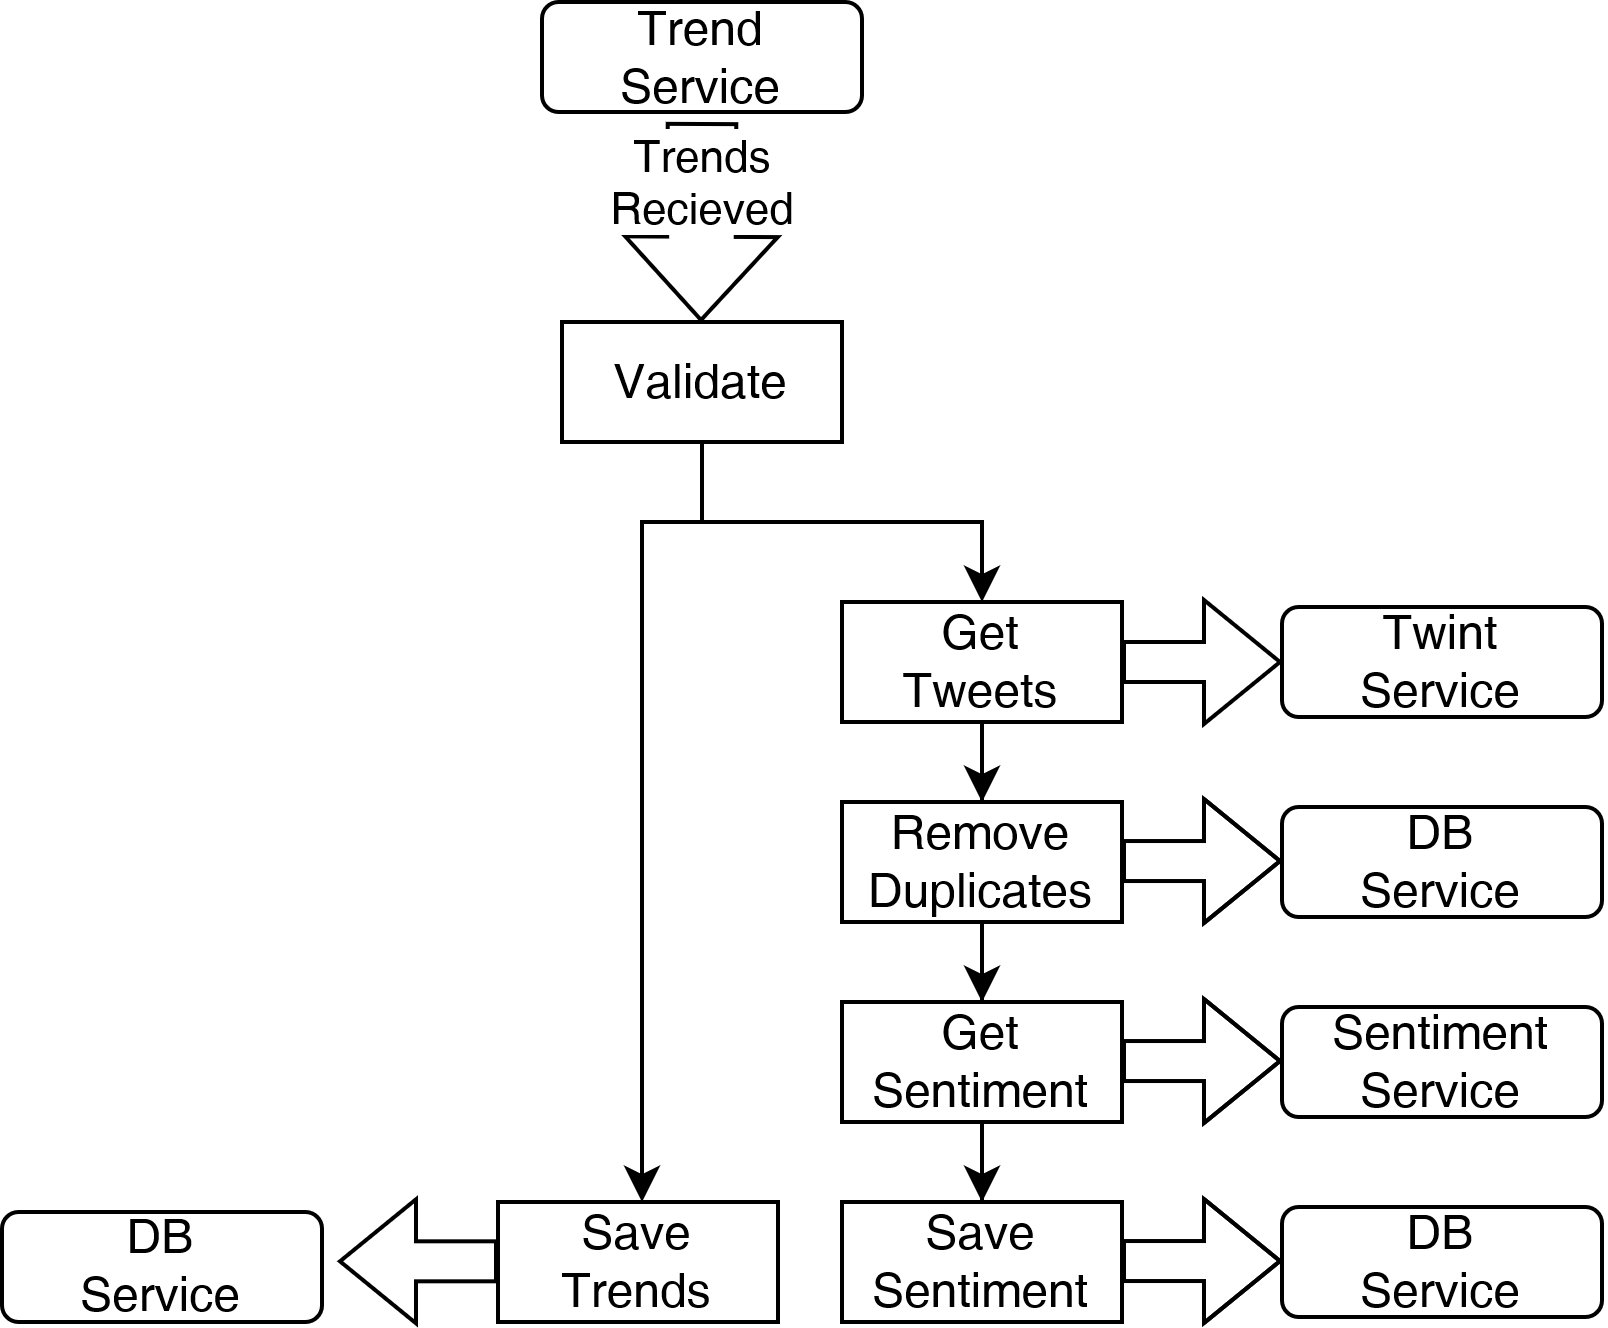
\includegraphics[width=0.5\textwidth]{Workflow.png}
    \caption{Standard Workflow}
\end{figure}


\section{Datenbank}
Alle Datenbankanfragen werden durch einen Datenbank-Service abstrahiert, der die Funktionen als gRPC-Schnittstelle anbietet.
Dabei laufen die Datenbank und der Datenbank-Service in jeweils einem eigenen Container.
Durch die gRPC-Schnittstelle können die Daten typsicher und plattform- sowie programmiersprachenunabhängig an den Datenbank-Service übergeben und von diesem zurückgeliefert werden.
\\
Vom Datenbank-Service werden folgende Funktionen angeboten:
\\
Zur Speicherung in die Datenbank:
\\
\smallskip
\textbf{Trends speichern (StoreTrends)}
\begin{itemize}
    \item Beschreibung: Speichert Trends in die Datenbank
    \item Parameter:
          \begin{itemize}
              \item Zeitstempel
              \item Liste von Trends mit folgenden Attributen:
                    \begin{itemize}
                        \item trendtype
                        \item name
                        \item country
                        \item placement
                        \item tweetVolume24
                    \end{itemize}
          \end{itemize}
    \item Rückgabe: Keine
\end{itemize}

\smallskip
\textbf{Sentiment speichern (StoreSentiment)}
\begin{itemize}
    \item Beschreibung: Speichert Sentiment in die Datenbank
    \item Parameter:
          \begin{itemize}
              \item Liste von Sentiments mit folgenden Attributen:
                    \begin{itemize}
                        \item Tweet
                        \item Sentiment
                        \item Topic
                    \end{itemize}
          \end{itemize}
    \item Rückgabe: Keine
\end{itemize}

Zum Laden aus der Datenbank:
\\
\smallskip
\textbf{Aktuelle Trends abrufen (GetCurrentTrends)}
\begin{itemize}
    \item Beschreibung: Lädt aktuelle Trends aus der Datenbank
    \item Parameter:
          \begin{itemize}
              \item Land
              \item Limit
          \end{itemize}
    \item Rückgabe:
          \begin{itemize}
              \item Zeitstempel
              \item Liste von Trends mit folgenden Attributen:
                    \begin{itemize}
                        \item Trendtyp
                        \item Name
                        \item Land
                        \item Platzierung
                        \item 24Stunden-Volumen
                    \end{itemize}
          \end{itemize}
\end{itemize}

\smallskip
\textbf{Vergangene Trends abrufen (GetRecentTrends)}
\begin{itemize}
    \item Beschreibung: Lädt vergangene Trends aus der Datenbank
    \item Parameter:
          \begin{itemize}
              \item Hashtag
              \item Land
              \item Startzeitpunkt (optional)
              \item Endzeitpunkt (optional)
          \end{itemize}
    \item Rückgabe:
          \begin{itemize}
              \item Liste an Trends mit folgenden Attributen:
                    \begin{itemize}
                        \item Zeitstempel
                        \item Liste von Trends mit folgenden Attributen:
                              \begin{itemize}
                                \item Trendtyp
                                \item Name
                                \item Land
                                \item Platzierung
                                \item 24Stunden-Volumen
                              \end{itemize}
                    \end{itemize}
          \end{itemize}
\end{itemize}

\smallskip
\textbf{Vorhandene Länder abrufen (GetAvailableCountries)}
\begin{itemize}
    \item Beschreibung: Lädt vorhandene Länder aus der Datenbank
    \item Parameter: Keine
    \item Rückgabe: Liste mit allen Ländern, die in der Datenbank vorhanden sind
\end{itemize}

\smallskip

\textbf{Trends mit vorhandenen Sentiment abrufen (GetTrendsWithAvailableSentiment)}
\begin{itemize}
    \item Beschreibung: Lädt Trends mit vorhandenen Sentiment aus der Datenbank, welche den Query String enthalten.
    \item Parameter:
          \begin{itemize}
              \item Query
              \item Limit
          \end{itemize}
    \item Rückgabe: Liste von Trendnamen
\end{itemize}

\smallskip
\textbf{Aktuelles Sentiment abrufen (GetCurrentSentiment)}
\begin{itemize}
    \item Beschreibung: Lädt aktuelles Sentiment (Mittel der letzten Stunde) aus der Datenbank
    \item Parameter:
          \begin{itemize}
              \item Trendname
          \end{itemize}
    \item Rückgabe: Sentiment
\end{itemize}

\smallskip
\textbf{Vergangene Sentiments abrufen (GetRecentSentiments)}
\begin{itemize}
    \item Beschreibung: Lädt vergangene Sentiments aus der Datenbank
    \item Parameter:
          \begin{itemize}
              \item Trendname
              \item Startzeitpunkt (optional)
              \item Endzeitpunkt (optional)
              \item Auflösung
          \end{itemize}
    \item Rückgabe: Liste der vergangenen Sentiments in Zeitabschnitt 
\end{itemize}

\smallskip
\textbf{DB auf Tweet prüfen (GetUniqueTweets)}
\begin{itemize}
    \item Beschreibung: Gibt zurück, welche Tweets noch nicht in der Datenbank sind
    \item Parameter: Liste an Tweet IDs
    \item Rückgabe: Liste an Tweet IDs
\end{itemize}

\smallskip

Vom Backend erzeugte Daten werden in einer MongoDB Datenbank gespeichert.
Dabei werden Trends zu bestimmten Zeitpunkten mit folgenden Feldern gespeichert:
\begin{itemize}
    \item Trendtyp
    \item Name
    \item Land
    \item Platzierung
    \item 24Stunden-Volumen
\end{itemize}
Für alle erfassten Tweets werden folgende Felder gespeichert:
\begin{itemize}
    \item Tweet-ID
    \item Sentiment
    \item Topic
    \item Zeitstempel
\end{itemize}

\section{Frontend}
%TODO

\section{Testing}
Um die Funktionalität des Backends zu garantieren wurden alle Backend-Dienste mit einem zur verwendeten Programmiersprache passenden Unit-Test Framework getestet.
Die Code-Converage liegt dabei bei jeden Dienst über 90\%.
Der Trend-,Twint- und Sentiment-Dienst wurden mit dem Python Unittest\cite{unittest} Framework getestet.\\
Der Conductor- und Datenbank-Dienst wurden mit dem NUnit\cite{nunit} Framework in einem Arrange-Act-Assert-Pattern getestet.
Das Frontend wurde noch nicht mit Unittests abgedeckt.

\begin{thebibliography}{0}
    \bibitem{microservices}Microservice-Frontend-Architekturen [Online] \url{https://www.sigs-datacom.de/uploads/tx_dmjournals/attermeyer_OTS_Microservices_Docker_16.pdf} (visited on Jun. 21, 2022)
    \bibitem{twitterapi}Twitter-API [Online] \url{https://developer.twitter.com/en/docs/twitter-api} (visited on Jun. 23, 2022)
    \bibitem{twint}TWINT - Twitter Intelligence Tool [Online] \url{https://github.com/twintproject/twint} (visited on Jun. 23, 2022)
    \bibitem{tweepy}Tweepy: Twitter for Python! (2020) [Online] \url{https://github.com/tweepy/tweepy} (visited on Jun. 23, 2022)
    \bibitem{bert}bert-base-multilingual-uncased-sentiment [Online] \url{https://huggingface.co/nlptown/bert-base-multilingual-uncased-sentiment} (visited on Jun. 23, 2022)
    \bibitem{textblob}TextBlob: Simplified Text Processing [Online] \url{https://textblob.readthedocs.io/en/dev/} (visited on Jun. 23, 2022)
    \bibitem{elsa}ELSA - An open source .NET Standard workflow library [Online] \url{https://elsa-workflows.github.io/elsa-core/} (visited on Jun. 25, 2022)
    \bibitem{unittest}Unittest - Unit testing framework [Online] \url{https://docs.python.org/3/library/unittest.html} (visited on Jun. 25, 2022)
    \bibitem{nunit}NUnit is a unit-testing framework for all .Net languages. [Online] \url{https://nunit.org/} (visited on Jun. 25, 2022)

    
\end{thebibliography}

\end{document}
